\section{Discussion}

\begin{table*} % Full width table (notice the starred environment)
	\caption{Example two column table with fixed-width columns.}
	\centering % Horizontally center the table
	\begin{tabular}{L{0.2\linewidth} L{0.2\linewidth} R{0.15\linewidth}} % Manually specify column alignments with L{}, R{} or C{} and widths as a fixed amount, usually as a proportion of \linewidth
		\toprule
		\multicolumn{2}{c}{Location} \\
		\cmidrule(r){1-2}
		East Distance & West Distance & Count \\
		\midrule
		100km & 200km & 422 \\
		350km & 1000km & 1833 \\
		600km & 1200km & 890 \\
		\bottomrule
	\end{tabular}
\end{table*}

\begin{figure} % Single column figure
	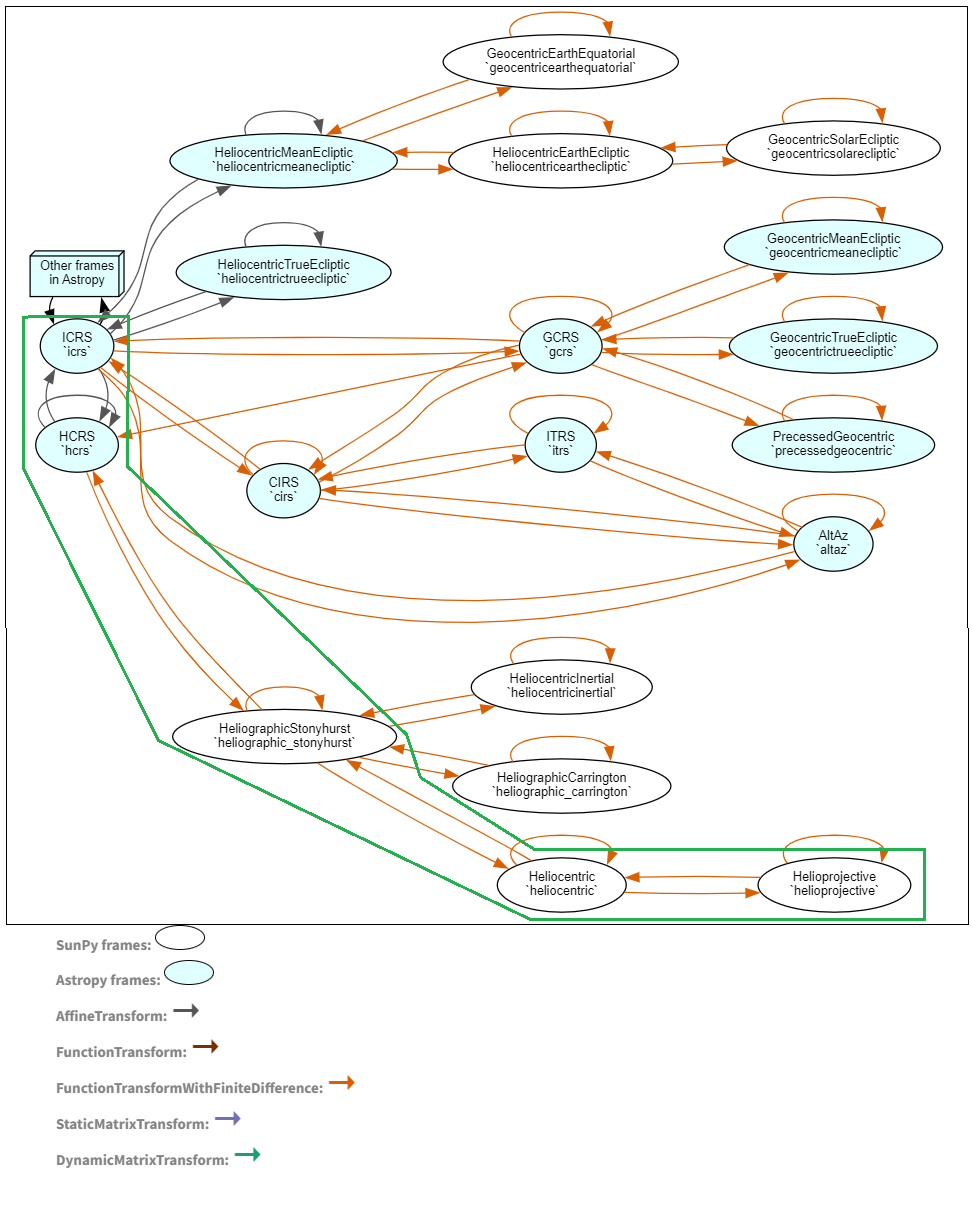
\includegraphics[width=\linewidth]{report/Figures/methods/coordinates.png}
	\caption{Anther of thale cress (Arabidopsis thaliana), fluorescence micrograph. Source: Heiti Paves, \href{https://commons.wikimedia.org/wiki/File:Tolmukapea.jpg}{https://commons.wiki-\\media.org/wiki/File:Tolmukapea.jpg}.}
	\label{fig:tcanther}
\end{figure}

\begin{figure*} % Two column figure (notice the starred environment)
	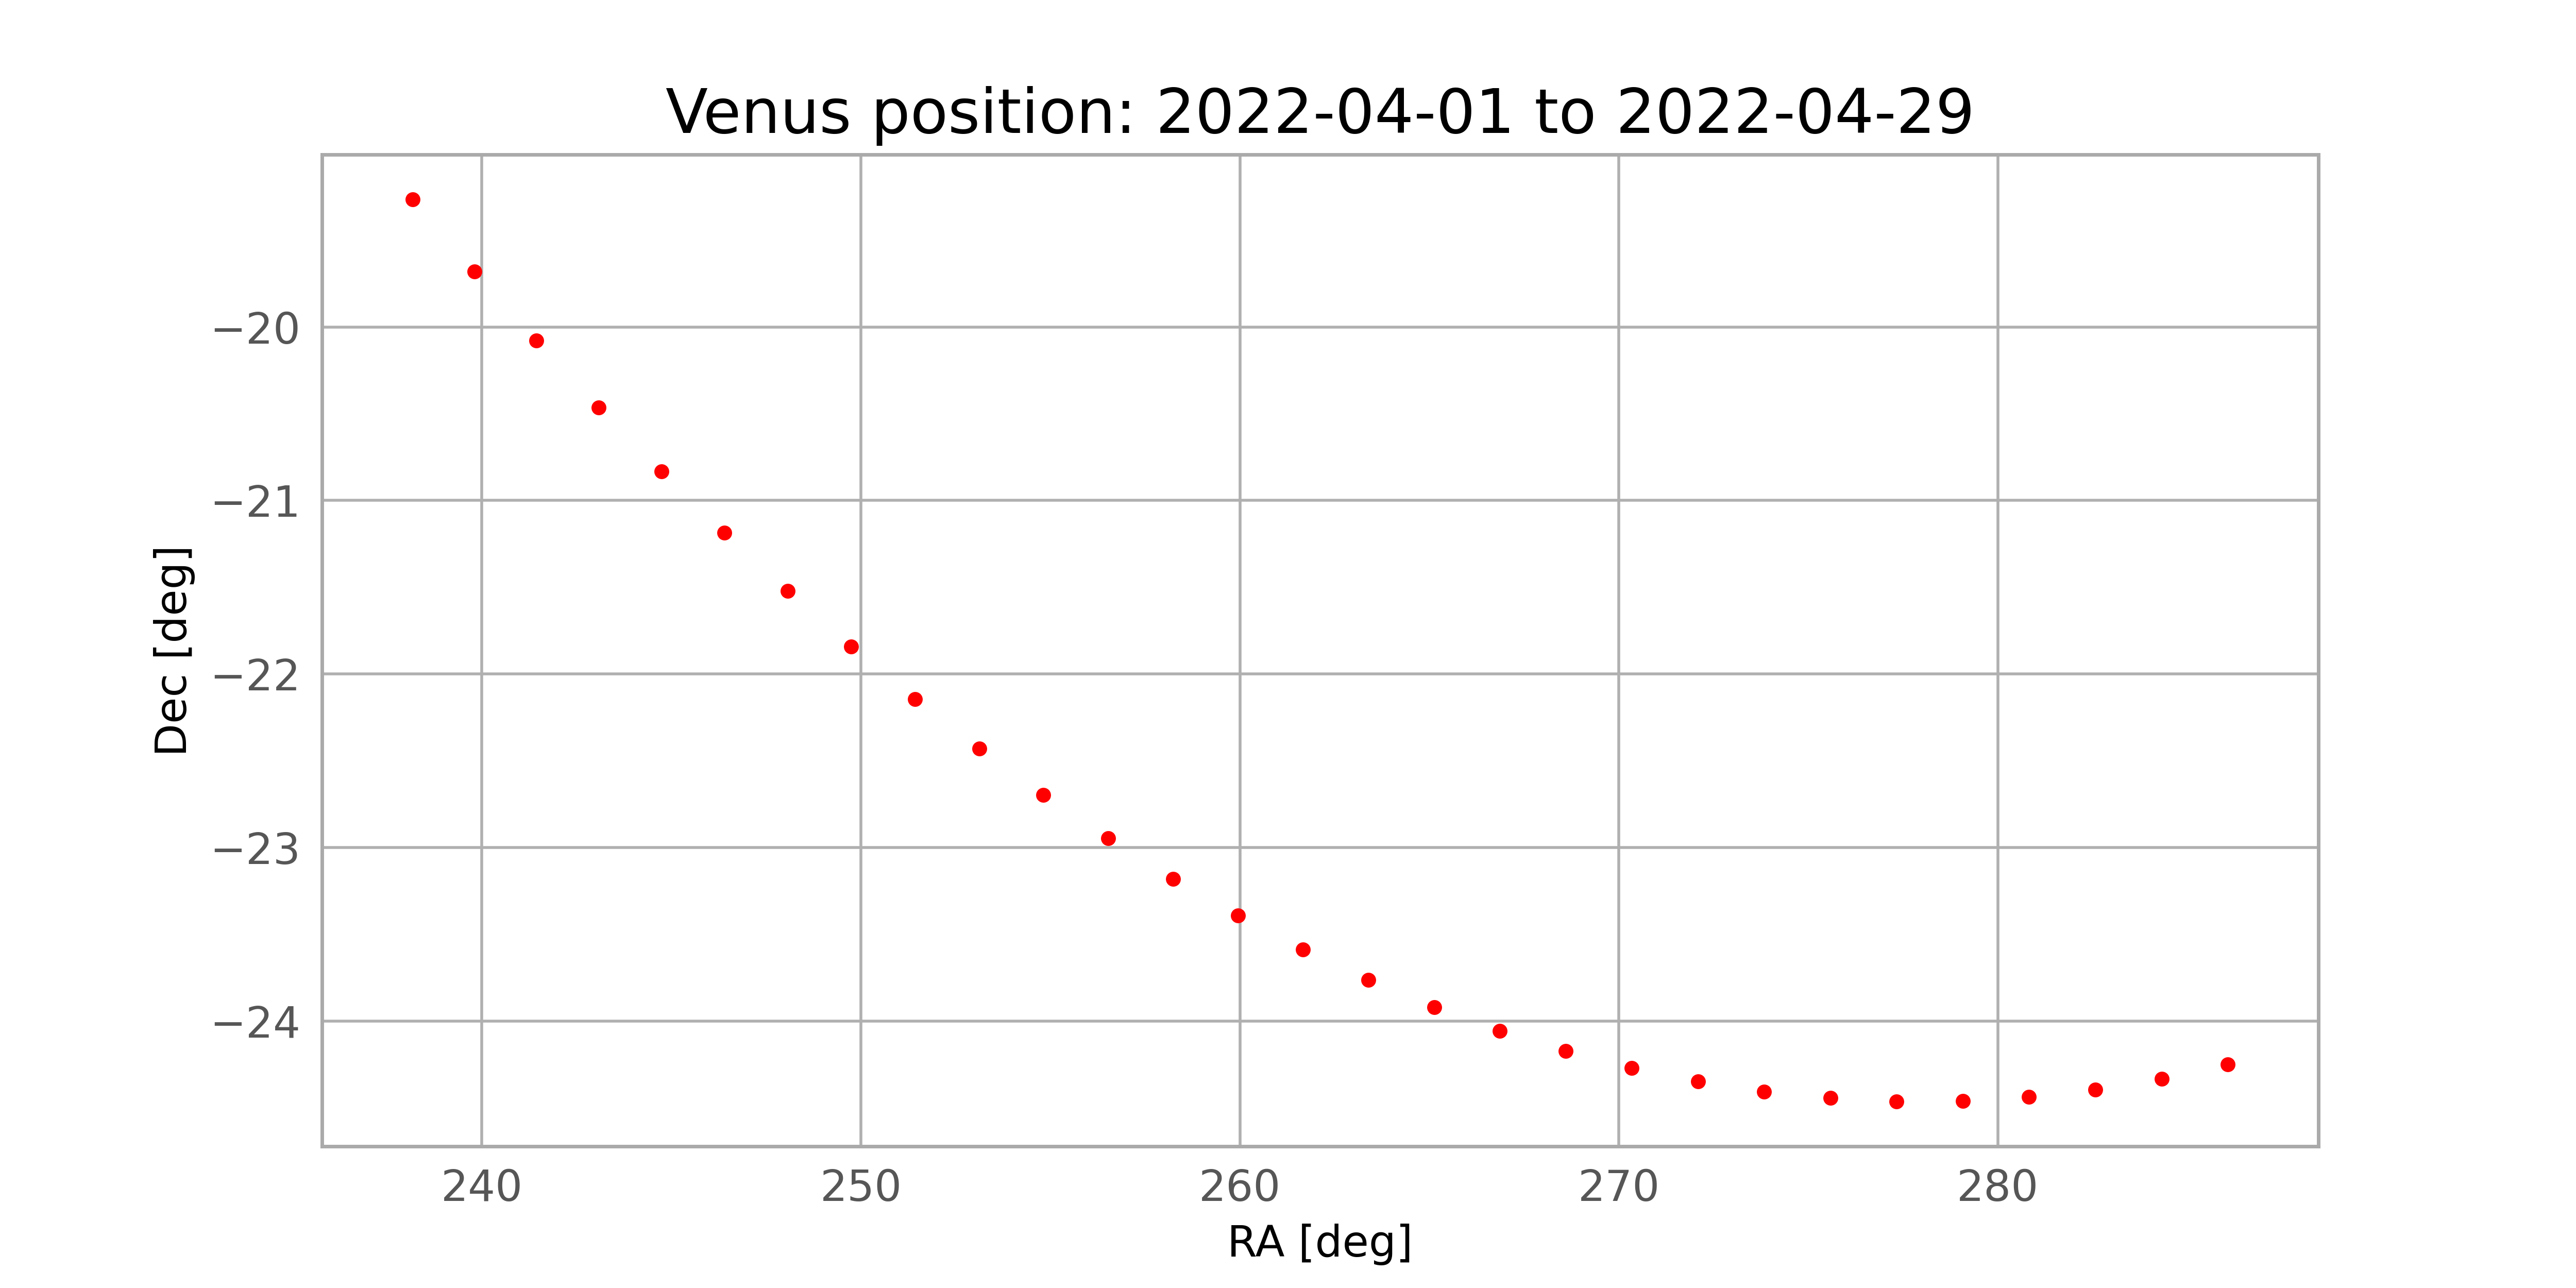
\includegraphics[width=\linewidth]{report/Figures/methods/Venus_position.png}
	\caption{Bovine pulmonary artery endothelial cells in culture. Blue: nuclei; red: mitochondria; green: microfilaments. Computer generated image from a 3D model based on a confocal laser scanning microscopy using fluorescent marker dyes. Source: Heiti Paves, \href{https://commons.wikimedia.org/wiki/File:Fibroblastid.jpg}{https://commons.wikimedia.org/wiki/File:Fibroblastid.jpg}.}
	\label{fig:bpartery}
\end{figure*}